\documentclass[a4paper, 12pt]{scrartcl}

\usepackage[utf8]{inputenc}
%\usepackage[ngerman]{babel}
\usepackage[T1]{fontenc}
\usepackage{amsmath}
\usepackage{braket}
\usepackage{amssymb}
\usepackage{graphicx}
\usepackage{wrapfig}
\usepackage{hyperref}
\usepackage{float} 
\usepackage{lmodern}

\author{Sebastian Steinhäuser}

\begin{document}

\tableofcontents
\newpage
\section{Viele Random-Walker auf dem freien Cluster mit Nahrung (2D)}
\subsection{Interaktion der Random-Walker}
Die einzelnen Random-Walker haben keine direkte Interaktion untereinander, es ist also insbesondere auch möglich, dass zwei (oder mehrere) Random-Walker auf der gleichen Position im Gitter sitzen. Der einzige Wechselwirkungseffekt der bei diesem Modell vorliegt ist, dass die Walker sich gegenseitig 'Nahrung wegessen' und somit die Umgebung eines anderen Walkers verändern und damit auch die Wahrscheinlichkeiten wohin der nächste Schritt ausgeführt wird. Es wurden zwei Zugversionen getestet, einmal ziehen alle Random-Walker zur selben Zeit und alternativ ziehen die Random-Walker sukzessive, also zuerst Random-Walker 1, gefolgt von Random-Walker 2 und so weiter. \\
\noindent Die Wahrscheinlichkeiten, wohin ein Random-Walker zieht werden wie in [XX] gemäß:
\begin{align}
p_{j \leftarrow i} = \frac{exp({F_j})}{\sum_j exp({F_j})}
\label{Wkeiten}
\end{align}
berechnet, wobei $F_j$ die Menge der Nahrung an Gitterplatz $j$ ist.

\subsection{Klassischer gegen sukzessiver Algorithmus}
Wie im vorigen Kapitel angekündigt, werden zwei verschiedene Zugvarianten der hungrigen Walker gegeneinander verglichen. Dies dient dazu um zu prüfen ob der im nachfolgenden beschriebene Effekt kein Artefakt der Zugversion ist.
\\
\noindent Es wird falls nicht anders angegeben über 1000 Läufe gemittelt. Da es 1000 Walker gibt mittelt man so über $10^6$ einzelne $msd$. Eine deutlich 'bessere' Statistik ist aus Gründer der Laufzeit beziehungsweise der Rechnerkapazitäten nicht möglich. Zudem erscheint die Anzahl an Samples ausreichend.
\\
\noindent Es stellt sich heraus, dass man ein nahezu identisches Ergebnis aus den beiden Monte-Carlo-Simulationen erhält. Der im nächsten Kapitel beschriebene Effekt ist daher stabil gegenüber der verwendeten Zugversion.
\\
\noindent Es wird im weiteren daher die zuerst vorgeschlagene Zugversion verwendet.

\begin{figure}[h!]
	\centering
	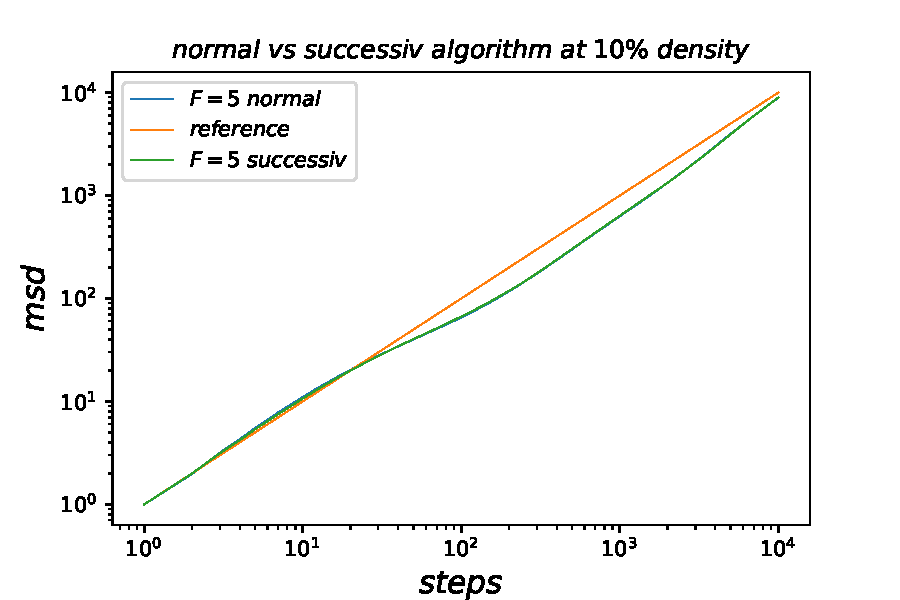
\includegraphics[scale=0.9]{suc.pdf}
	\caption{Monte-Carlo Ergebnisse der beiden Zugversionen für das $msd$ von $1000$ Walkern auf einem (für $F\neq0$) mit Nahrung bestückten freien $100\times 100$ Gitter (also einer Dichte von 10\%). Die Kurve 'reference' bezeichnet: $msd(t)=t$.}
\end{figure}

\newpage 

\subsection{Auftreten eines streng subdiffusiven Regimes}
Durch Monte-Carlo-Simulation wurde das $msd$ für ein $100 \times 100$ Gitter und $1000$ Random-Walkern ermittelt. Es lässt sich für $F=2$ und besonders für $F=5$ ein streng subdiffusives Regime erkennen, das heißt ein Bereich, in dem das $msd$ kleiner ist als das $msd$ des freien Random-Walks ohne Nahrung ($F=0$) und mit geringerem Diffsuionsexponenten steigt (also anormale Diffusion vorliegt). Beachte, das wenn nur ein Diffusionsexponent $\nu < 0.5$ vorliegt von (nicht streng) subdiffusiv gesprochen wird.\\
\noindent Zudem liegt zu Beginn des Prozess Superdiffusion vor, das heißt der Random-Walker ist 'schneller' als der freie Random-Walk ($msd(t)=t$).\\
\noindent Der superdiffusive Bereich ist zu erwarten und lässt sich leicht erklären. Zu Beginn sind die Walker im mittel noch mehrere Gitterplätze voneinander entfernt und sehen nur ihren eigenen Zug und meiden daher (je höher $F$ ist desto stärker) in die entgegengesetzte Richtung zurückzukehren, ähneln also dem SAW. \\
\noindent Der Großteil dieses Kapitels beschäftigt sich mit der Erklärung des streng subdiffusiven Bereichs, welcher zunächst sehr merkwürdig erscheint und im Gegensatz zum superdiffusiven Regime nicht (naiv) zu erwarten ist.
\\
\noindent Zur Simulation muss erneut bemerkt werden, das die Nahrung (nach Besuch eines Walkers) aus der 'originalen' Matrix und somit auch aus allen periodischen Kopien gelöscht wird. Die Walks sind dementsprechend auf die Länge der Boxgröße zu beschränken um starken finite size Effekten vorzubeugen. Es wird zudem über alle Walker gemittelt um das $msd$ zu berechnen.
\\
\noindent In den nachfolgenden Unterkapiteln wird (hauptsächlich) der $F=5$ Fall bei 10\% Dichte untersucht, um eine Erklärung für das streng subdiffusive Regime zu finden. 

\noindent Die nachfolgende Abbildung zeigt das oben diskutierte $msd$ von 1000 Walkern auf einem mit Nahrung bestückten freien $L=100$ Gitter. Im Fall $F=5$ ist deutlich zu sehen, wie rund die ersten 20 Schtritte superdiffusiv sind und danach in ein streng subdiffusives Regime gewechselt wird. Die $F=0$ Kurve kann als Referenz angesehen werden, da ohne Nahrung absolut keine Wechselwirkung mehr zwischen den einzelnen Walkern besteht, womit ein normaler zweidimensionaler Random-Walk ausgeführt wird.

\begin{figure}[h!]
	\centering
	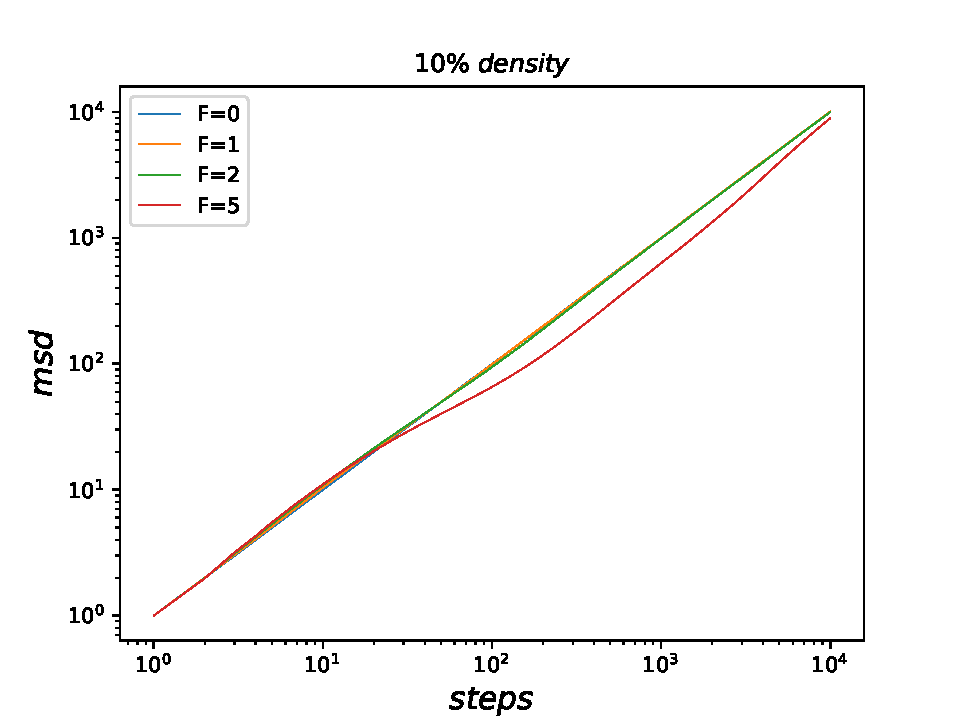
\includegraphics[scale=0.9]{mult_food.pdf}
	\caption{\label{vieleF}Monte-Carlo Ergebnisse für das $msd$ von $1000$ Walkern auf einem (für $F\neq0$) mit Nahrung bestückten freien $100\times 100$ Gitter (also einer Dichte von 10\%).}
\end{figure}

\newpage

\subsection{Fraktale Dimension der Nahrungsverteilung}
Der erste Versuch zur Erklärung des streng subdiffusiven Verhaltens der Random-Walker ist es, numerisch die fraktale Dimension der Nahrungsverteilung zu bestimmen, denn die Walker laufen mit sehr hoher Wahrscheinlichkeit auf mit Nahrung besetzten Feldern des Gitters (der Matrix) und somit hat die Struktur der Nahrungsverteilung einen Einfluss auf das $msd$ der Walker. Zudem wird der Anteil an vorhandener Nahrung gegen die MC-Schritte aufgetragen, die Nahrung wird auf den ersten Schritt normiert, das heißt es wird durch die mittlere Dichte der freien Felder zum Quadrat geteilt.
\subsubsection{Die Box-Counting-Methode}
Zur Bestimmung der fraktalen Dimension wird die sogenannte Box-Counting-Methode verwendet.\footnote[1]{\url{https://en.wikipedia.org/wiki/Box\_counting} 23.12.2019} 
\\
\noindent Es werden sukzessive Boxen von der Größe $l=2^n$ , $l=2^{n-1}$ , ... , $l=2$ gebildet und jeweils die Anzahl der mit Nahrung belegten Felder gezählt. Die fraktale Dimension ist dann der Exponent bzw. hier bei doppelt logarithmischer Auftragung der Vorfakter wie die Anzahl der Nahrungseinheiten mit der Boxgröße skalieren. Hier wurde eine leichte Veränderung des Codes von Nicolas P. Rougier verwendet\footnote[2]{\url{https://gist.github.com/rougier/e5eafc276a4e54f516ed5559df4242c0} 23.12.2019}.
\\
Genauere Details und mögliche Implementierung dieser Methode können dem nachfolgenden Python3 Code entnommen werden.
\begin{figure}[h!]
	\centering
	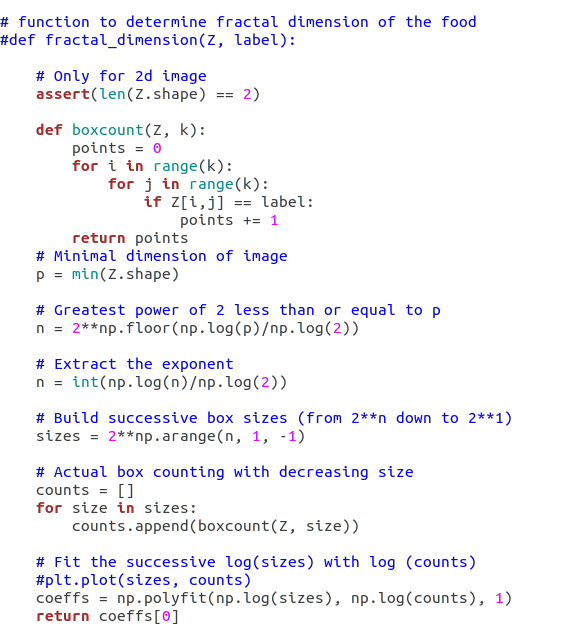
\includegraphics[scale=0.8]{fractal.png}
	\caption{Python3 Code für das Box-Counting zur Bestimmung der fraktalen Dimension der Nahrungsverteilung.}
\end{figure}

\newpage

\subsubsection{Ergebnisse der Box-Counting Analyse}
Die nachfolgende Abbildung zeigt die Ergebnisse der Box-Counting Analyse zur fraktalen Dimension der Nahrungsverteilung. Es ist (abseits von numerischen Schwankungen) keine Veränderung zu erkennen, da die Walker gleichmäßig in der Marix verteilt sind und somit auch die 'Fressspuren' gleichmäßig über die Box verteilt sind, das heißt in einer doppelt so großen Box ($ l \rightarrow 2l$) sind viermal so viele 'Fressspuren' und daher ist die numerisch bestimmte fraktale Dimension die gesamte Zeit ca. $2$.
\\
\noindent Die Box-Counting Methode wird also im weiteren Verlauf nicht mehr verwendet un wurde hier nur zur Vollständigkeit diskutiert. 
 
\begin{figure}[h!]
	\centering
	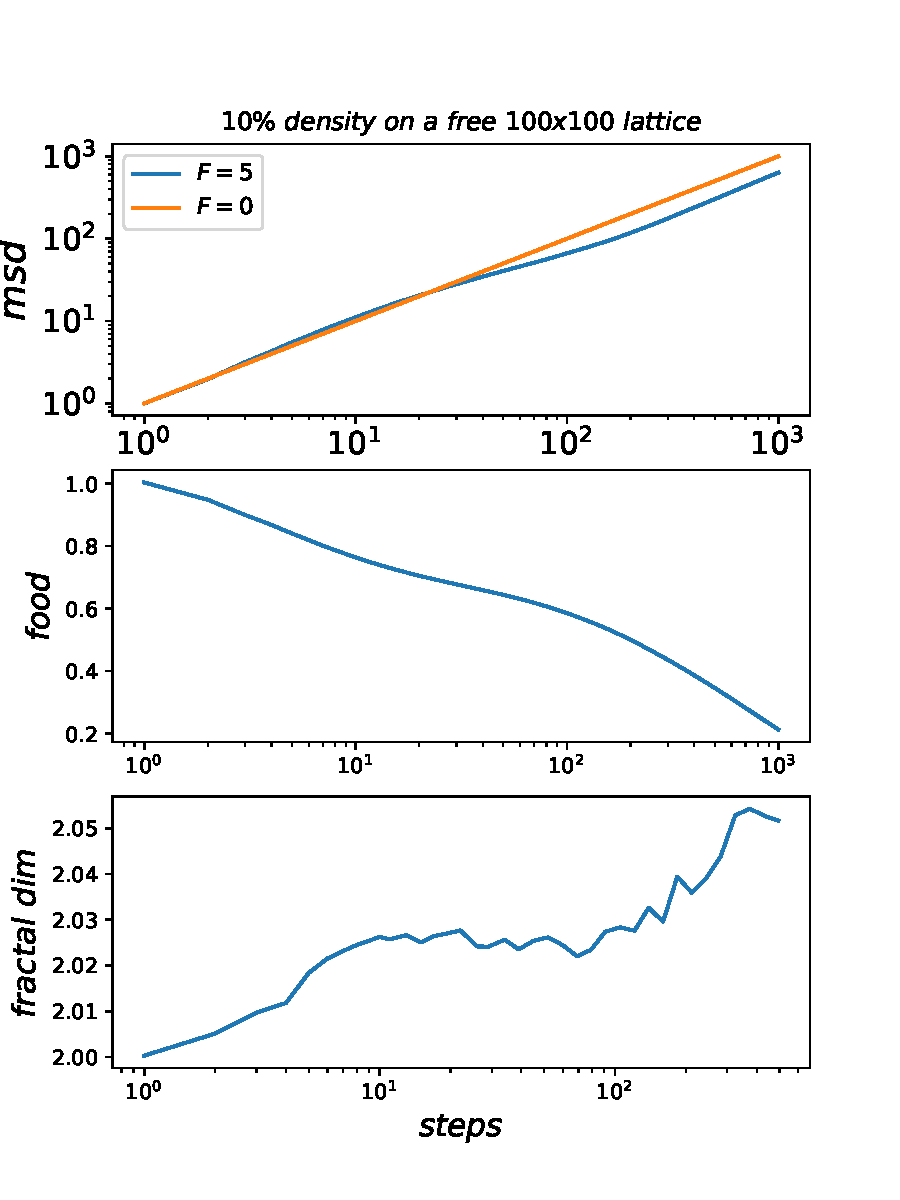
\includegraphics[scale=0.75]{10fractal.pdf}
	\caption{Ergebniss der Box-Counting Analyse bei 1000 Walkern auf dem $100\times 100$ Gitter mit $F=5$.}
\end{figure}

\newpage
\subsubsection{Nahrungsvorrat}
\noindent Man sieht ebenfalls in obiger Abbildung, das während des Wechsels von superdiffusiv zu streng subdiffusiv weniger Nahrung 'gegessen' wird. Während der superdiffusiven Phase wird natürlich viel Nahrung gegessen, da sich die Walker nur zu mit Nahrung besetzten Feldern ziehen und im Mittel mit keinen anderen Walker interagieren (durch 'wegessen' von Nahrung). In der streng subdiffusiven Phase wird durch die langsamere Ausbreitung entsprechend auch weniger Nahrung gegessen. Es lässt sich also eine Korrelation zwischen der dem Diffusionsexponenten und dem Sinken des Nahrungsvorrats erkennen.
\newpage
\noindent Ziel der nachfolgenden Kapitel ist es einen Zusammenhang zwischen der Gestalt des Nahrungsvorrats und dem Übergang von superdiffusivem nach streng subdiffusivem $msd$ zu schaffen. Denn es ist klar, das dieser Übergang nur durch die Nahrungsverteilung entstehen kann, da sie die einzige Interaktion der ansonsten nicht-wechselwirkenden Walker ist.

\subsection{Vergröberte Dichtekorrelation der Walker}
\noindent Um zu prüfen, wie sich der Abstand der Walker zueinander mit der Anzahl an Schritten verändert, wird eine vergröberte Dichtematrix eingeführt. Dazu wird die bisherige \newline $100\times 100$-Matrix in $100$ $10\times 10$-Matrizen zerlegt und es wird die Besetzungszahl jeder dieser $10\times 10$-Matrizen in eine weitere $10\times 10$-Matrix geschrieben. Diese Matrix enthält nun die vergröberte Dichte der 100 ($10\times 10$)Blöcke aus denen die ursprüngliche Matrix besteht. 
\\
\noindent Das bedeutet wir haben zu jedem Zeitschritt $i$ eine Matrix $\rho$ welche die Besetzungszahl der Blöcke enthält, um eine über den 'Aufpunkt' gemittelte Abstands-Korrelation zu erhalten bildet man (zu fester Zeitschritt $i$):
\begin{equation}
\hat{corr_i}(\Delta x,\Delta y) = \sum_{x_0,y_0}\rho_i(x_0,y_0)\cdot\rho_i(x_0+\Delta x,y_0+\Delta y)\ ,
\end{equation}
anschließend bietet es sich an auf $\hat{corr_1}(0,0)$ zu normieren (damit Plots von 1 aus starten), also:
\begin{equation}
corr_i(\Delta x,\Delta y) = \frac{ \hat{corr_i}(\Delta x,\Delta y) }{ \hat{corr_1}(0,0) } \ .
\end{equation}
Die Implementierung sieht zu jeder fixen Zeit $i$ wie folgt aus, wobei $n$ hier eine Schleife über alle $N$ Walker ist.
\vspace{0.3cm}
\begin{figure}[h!]
	\centering
	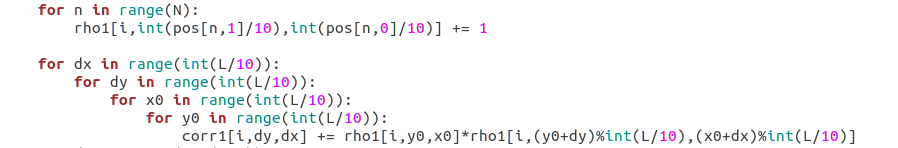
\includegraphics[scale=0.7]{corrcode.png}
	\caption{Implementierung der Korrelationsmatrix $\hat{corr_i}(\Delta x,\Delta y)$ zur Zeit $i$.}
\end{figure}

\newpage

\subsubsection{Selbstkorrelation}
\noindent Im folgenden wird $corr_i(0,0)$ als Selbstkorrelation eines Blocks bezeichnet, diese Größe gibt Auskunft über die die Verteilung der Walker auf die Blöcke. Dies lässt sich leicht an einem kleinen Beispiel einsehen, man stelle sich eine $3\times 3$ Matrix vor wo auf jedem Feld ein Walker sitzt, man erhält $\hat{corr}(0,0)=9$, befinden sich hingegen auf nur 3 Feldern je 3 Walker so ist $\hat{corr}(0,0)=27$. Das normieren skaliert nur die Achse, laufen Walker zusammen so steigt die Selbstkorrelation, nähern sich die Walker einer Gleichverteilung, so sinkt die Selbstkorrelation etwa auf 1, da anzunehmen ist (bei kleinen und mittleren Dichten wie sie bisher besprochen sind), dass nach einem Schritt die Walker noch Gleichverteilt sind, da sie noch nicht (indirekt über Nahrung) interagiert haben.
\\
\noindent Es wird die Selbstkorrelation für das bisherige 'Standardsystem' von 1000 Walkern auf dem $L=100$ Gitter vorgestellt. Dazu wird einmal wie oben erklärt das Gitter in 100 $10\times 10$ Blöcke unterteilt und einmal (völlig analog) in 400 $5\times 5$ Blöcke um eine feinere Auflösung zu erhalten. Leider wird die Kurve bei kleineren Blöcken (bei gleicher Sampleanzahl) weniger glatt, denn die Schwankungen sind natürlich größer, da Walker leichter am Rand des Blocks sich befinden können und somit wechseln Walker in diesem Fall leichter den Block. Eine starke Erhöhung der Anzahl von Samples ist leider (aus Gründen der Laufzeit) nicht möglich. Man erkennt jedoch trotzdem auch in dieser Variante, das Zusammenlaufen der Walker. 
\\
\noindent Man erkennt in beiden Versionen ein Ansteigen der Selbstkorrelation im streng subdiffusiven Bereich, das bedeutet, dass die Walker zusammenlaufen. Wenn der Nahrungsvorrat 'aufgegessen' ist bewegen sich die Walker wieder normal diffusiv und die Selbstkorrelation fällt wieder auf (ungefähr) 1. Im superdiffusiven Bereich bleibt die Selbstkorrelation wie zu erwarten auf (ungefähr) 1, da die Walker sich ja in kurzen Zeiten nicht sehen und nicht interagieren.
\\
\noindent Es lässt sich also sagen, dass es sich bei dem Übergang von Superdiffusion nach strenger Subdiffusion um einen Lokalisierungseffekt der Walker handelt. 
\\
\noindent Es bleibt aber zunächst offen wieso die Walker zusammenlaufen und auch der Einfluss auf das $msd$ ist unklar.

\begin{figure}[h!]
	\centering
	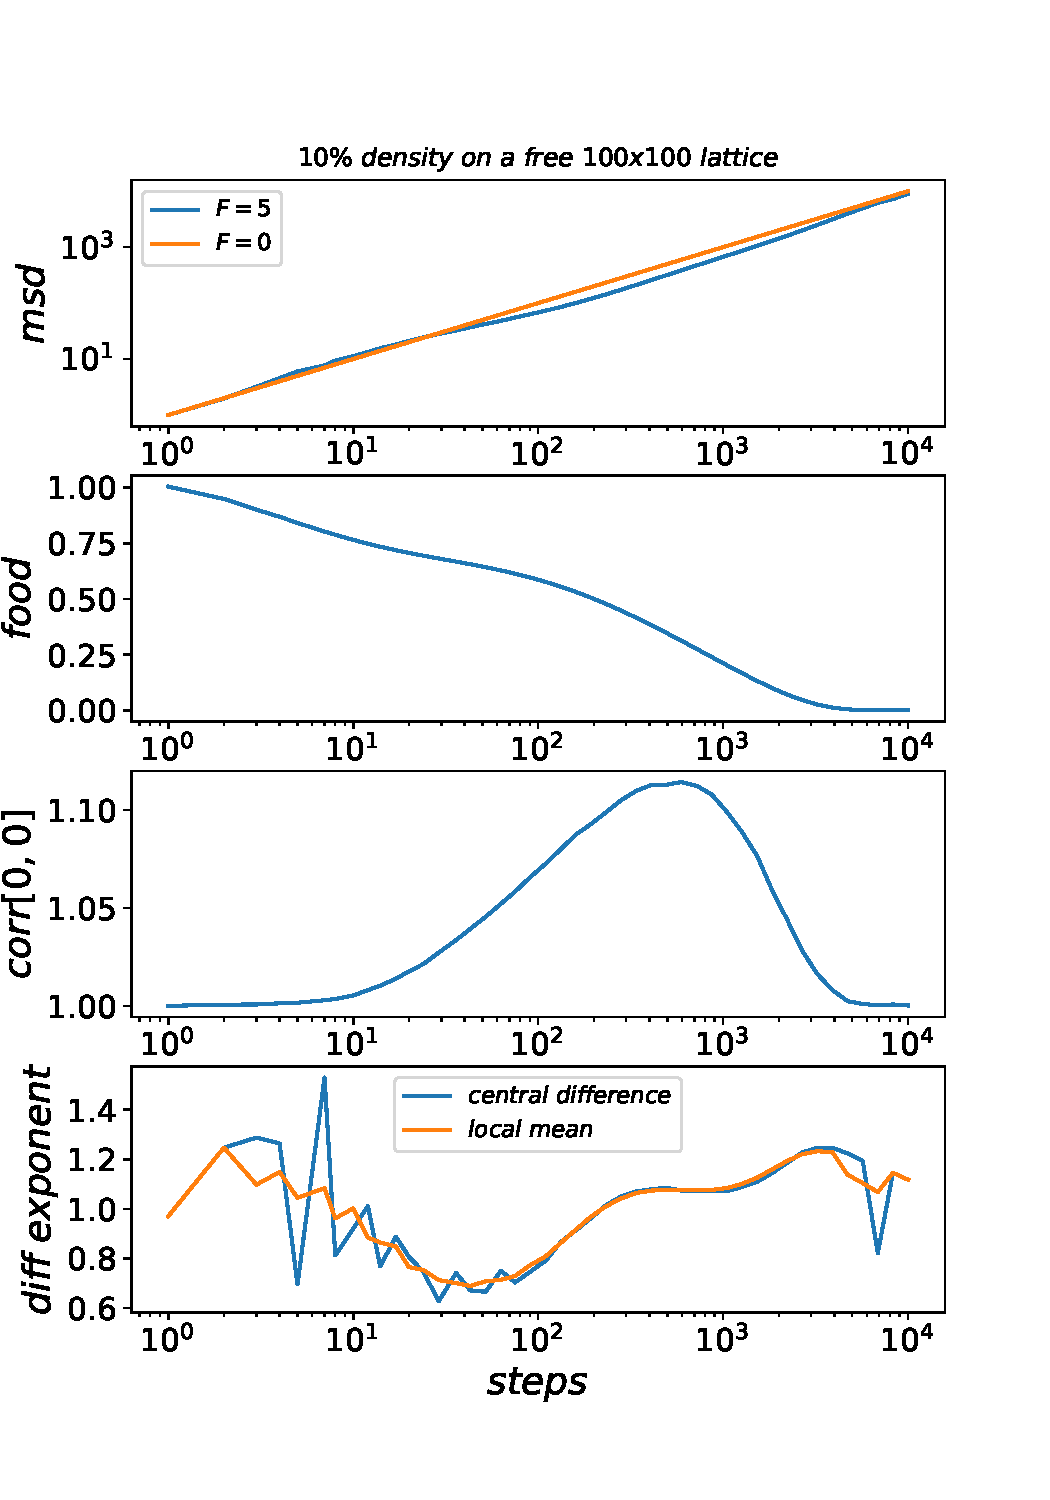
\includegraphics[scale=0.8]{corr1.pdf}
	\caption{Selbstkorrelation für $10\times 10$ Blöcke.}
\end{figure}

\newpage

\subsubsection{Korrelation mit benachbarten Blöcken}

In diesem Abschnitt wird die Korrelation zu benachbarten Blöcken untersucht, dabei ist es unwesentlich, ob $\Delta x$ oder $\Delta y$ zu festen Zeitschritten $t$ variiert wird, aufgrund der Symmetrie des Systems (Invarianz unter Drehungen um $\pi/2$). Es wird in nachfolgenden Plots daher stellvertretend für beide Möglichkeiten $\Delta x$ variiert.

\begin{figure}[h!]
	\centering
	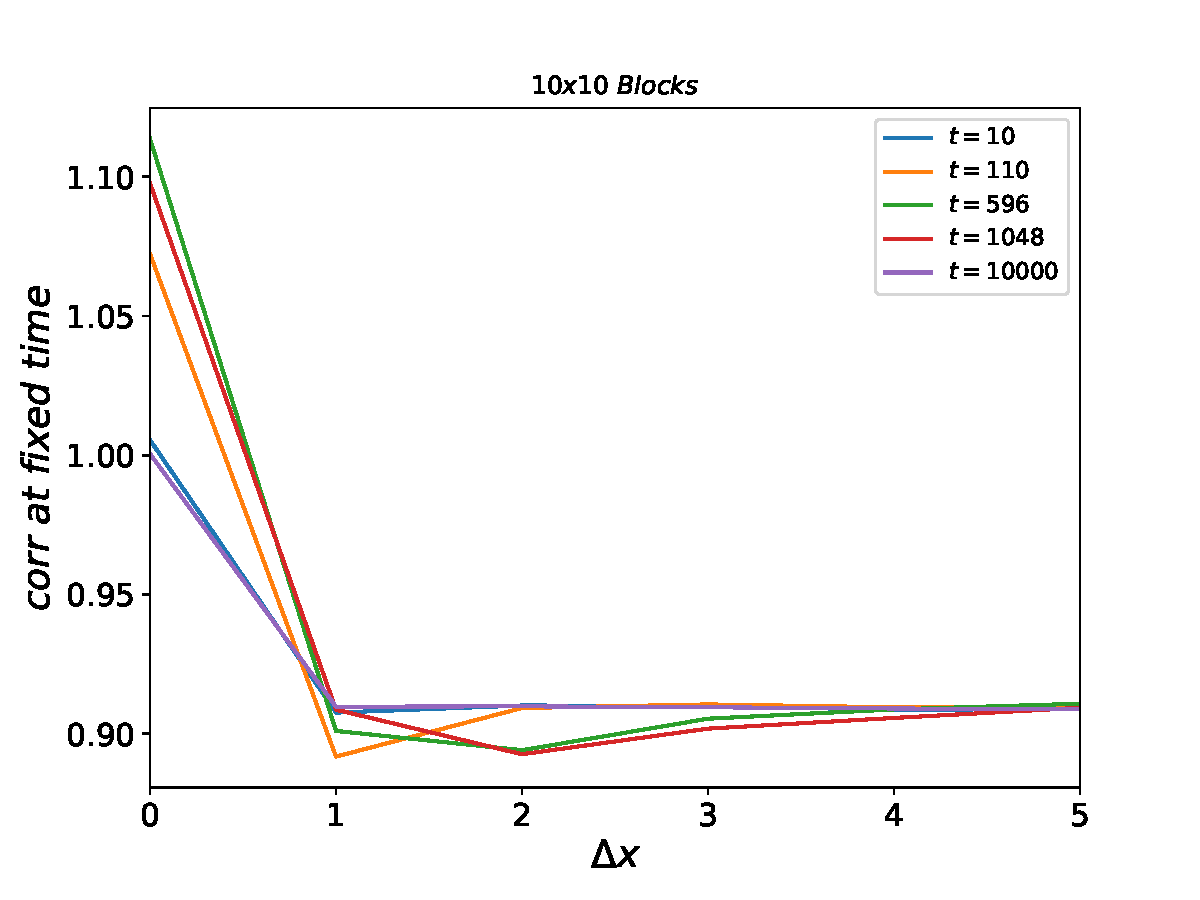
\includegraphics[scale=0.8]{corr10.pdf}
	\caption{Korrelation zu benachbarten Blöcken für eine Blockgröße von $10\times 10$.}
\end{figure}

\noindent Man erkennt, dass kurze und lange Zeiten erneut das gleiche Korrelationsverhalten haben, wie es sich nach dem vorigen Abschnitt schon vermuten lies. Wie zuvor sieht man die Steigung der Selbstkorrelation im streng subdiffusiven Bereich (also nach etwa 100 bis 1000 MC-Schritten), damit einhergehend fällt die Korrelation mit dem benachbarten Block. Man kann also sagen, dass die Teilchen aus den Nebenblocks zusammenwandern. Viele Blocks weiter (also hier 5) ändert sich die Korrelation nicht, da wie Walker nicht so weit laufen, zum Beispiel ist die Wurzel aus dem $msd$ zu $t=1048$ etwa $\sqrt{msd(1048)} \approx 30$, somit ist der Walker erst ungefähr 3 Blöcke weiter. 


\begin{figure}[h!]
	\centering
	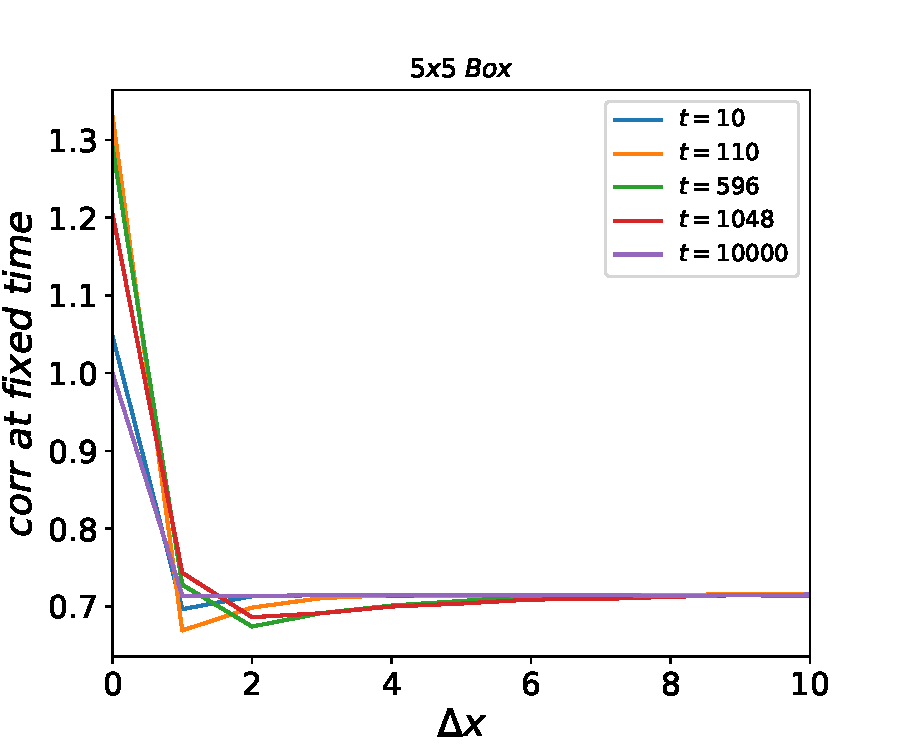
\includegraphics[scale=1]{corr5.pdf}
	\caption{Korrelation zu benachbarten Blöcken für eine Blockgröße von $5\times 5$.}
\end{figure}

\subsection{Autokorrelation der Schritte}
Da das $msd$ einen streng subdiffusive Bereich hat, liegt die Vermutung nahe, das die Walker 'zurückgezogen' werden zu ihren Startpunkt. Um diese Vermutung zu Untersuchen kann die folgende Korrelationsfunktion $g_{t_0}(\tau)$ gebildet werden. Es wird zuerst das (euklidische) Skalarprodukt zwischen dem Schrittvektor $\hat{e}(t_0)$ zur Zeit $t_0$ und dem Schrittvektor \break $\hat{e}(t_0+\tau)$ zur Zeit $t_0 + \tau$ eines Walkers berechnet und anschließend über alle Walker und alle Samples gemittelt, also bezeichnet $\langle \dots \rangle$ eine Ensemblemittelung. \\
\noindent Es ist demnach:
\begin{align}
g_{t_0}(\tau) = \langle \hat{e}(t_0+\tau) \cdot \hat{e}(t_0) \rangle\ .
\end{align}
Bei einem klassischen Random-Walk ist $g_{t_0}(\tau \neq 0)= 0$ für alle $t_0$ und natürlich gilt immer $g_{t_0}(\tau = 0)= 1$ denn $\hat{e}(t_0)$ ist einer der vier Einheitsvektoren $\pm \hat{e}_x,\ \pm \hat{e}_y$.
\\
Offensichtlich ist $g_{t_0}(\tau)$ positiv wenn mehr Schritte zur Zeit $t_0+\tau$ in als entgegen der Richtung des Schrittes zur Zeit $t_0$ gegangen sind und negativ anders herum. 
\\
\noindent Würden die Walker also 'zurückgezogen' werden, so würde man dies an einem negativen $g_{t_0=0}$ zu Zeiten der strengen Subdiffusion erkennen können. 

\begin{figure}[h!]
	\centering
	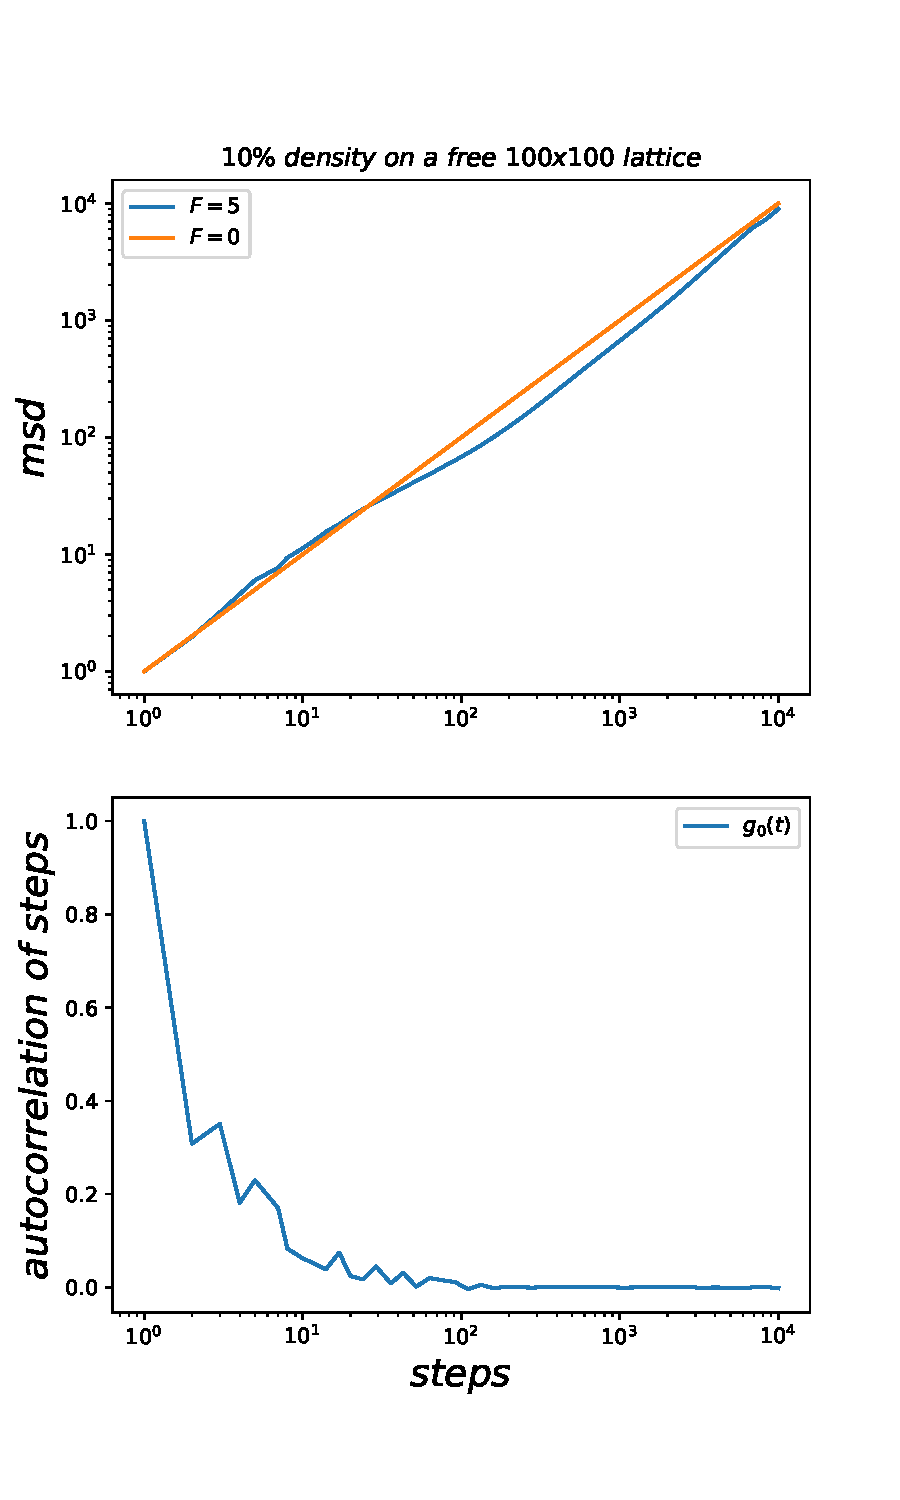
\includegraphics[scale=0.75]{autocorr.pdf}
	\caption{Autokorrelation der Schritte im Vergleich mit dem $msd$.}
\end{figure}

\clearpage

\subsection{'Fressspuren als Wände'}
Um zu klären, wieso das $msd$ bei $F=5$ einen streng subdiffusiven Bereich besitzt schaut man sich zunächst die Nahrungsmatrix zum Zeitpunkt $t=100$ an. Es ist zu sehen, dass die Fressspuren die Matrix in viele kleine Cluster teilt. 

\begin{figure}[H]
	\centering
	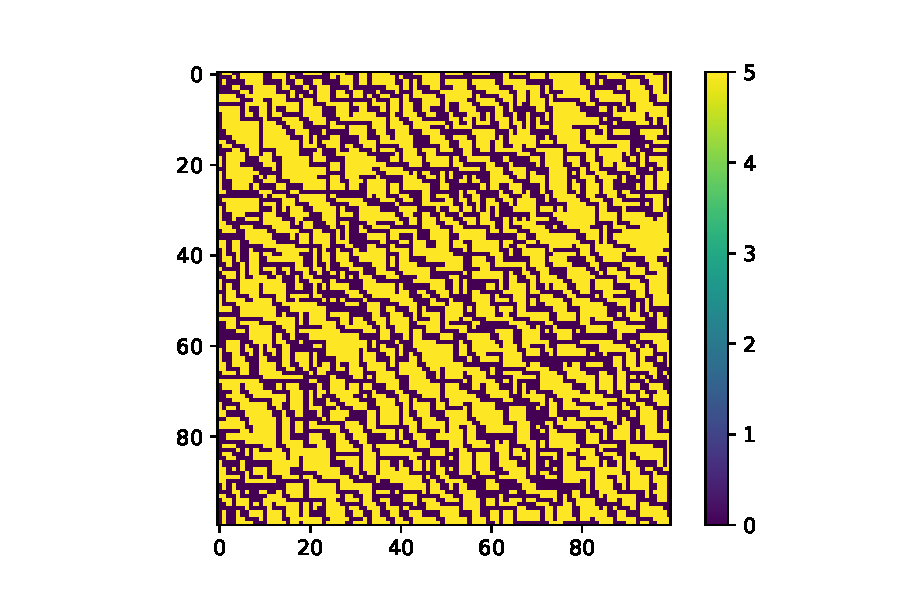
\includegraphics[scale=0.8]{usedmat.pdf}
	\caption{Nahrungsverteilung nach 100 MC-Schritten, also in der subdiffusiven Phase. Gelb = Nahrung, Schwarz = keine Nahrung}
\end{figure}


\noindent Die hungrigen Walker gehen nahezu sicher (wenn es möglich ist) auf Felder mit Nahrung: denn angenommen eins der vier benachbarten Felder enthält Nahrung und die anderen 3 nicht, so beträgt die Wahrscheinlichkeit auf das mit Nahrung besetzte Feld zu gehen gemäß Gleichung \ref{Wkeiten} $\ \frac{e^5}{e^5 + 1+ 1+1} \approx 0.98$. Somit wirken die Fressspuren wie eine Art Wand, falls Nahrung in der Nähe ist. Die Walker werden also auf die kleinen Nahrungscluster 'eingeschlossen' bis diese 'aufgefressen' sind.


\subsubsection{Minimalmodel eines Walkers auf einem Nahrungsquadrat}\label{minimalmodell}
Ein leicht zu verstehendes und auch leicht zu implementierendes Minimalmodell ist es einen einzelnen Walker in die Mitte eines kleinen mit Nahrung besetzten Quadrates innerhalb einer größeren Matrix zu setzen. Hier wird zum Beispiel in die Mitte einer $L=100$ Matrix ein $l=20$ Quadrat mit Nahrung belegt (das heißt auf die x und y Indices 40 bis einschließlich 59), der Walker startet bei $x_0=y_0=50$.

\begin{figure}[H]
	\centering
	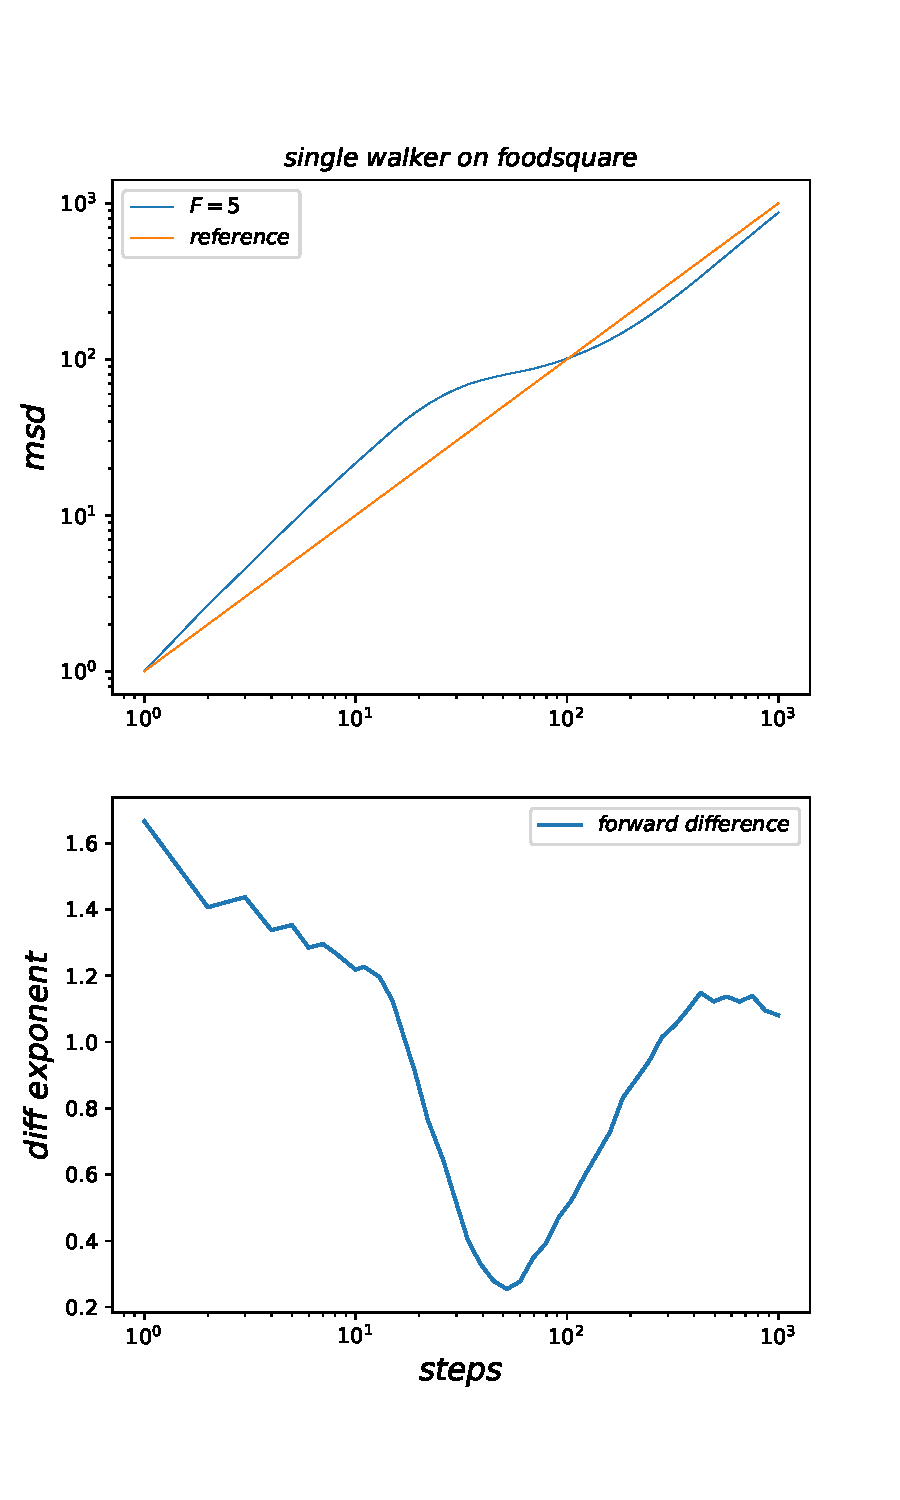
\includegraphics[scale=0.7]{single_walker_on20x20.pdf}
	\caption{Ergebniss der MC-Simulation des oben vorgestellten Minimalmodells. Es wurde über $10^5$ Samples gemittelt.}
\end{figure}


\noindent Es ist in der nachfolgenden Abbildung zu sehen, dass der Walker bei etwa $\sqrt{msd} \approx 10$ streng subdiffusiv wird, dies passt genau mit dem Erreichen von dem Rand des Nahrungsquadrat zusammen. Nach ungefähr 200 bis 300 MC-Schritten läuft der Walker wieder in fast diffusiv, da er sich 'freigefressen' hat, das Nahrungsquadrat ist nahezu leer und der Walker hat kein mit Nahrung benachbartes Feld um sich. 
\\
\noindent Zudem erkennt man an der numerischen Ableitung, beziehungsweise am daraus bestimmten Exponenten, dass das $msd$ fast konstant wird. Der (doppelte) Diffusionsexponent sinkt bis auf ungefähr $0.25$ ab, was eine sehr stark annormale Diffusion bedeutet.
\\
\noindent Das streng subdiffusive Verhalten lässt sich also auf diese Weise erklären. Da die vielen Walker auch nicht alle in gleich großen Nahrungsclustern 'eingeschlossen' sind tritt der Effekt (wie man am Vergleich der Exponenten erkennen kann) natürlich weniger stark auf.
\\
\noindent Nachfolgende Abbildungen zeigen, dass der Effekt sich (zeitlich) verschieben lässt, wenn das Nahrungsquadrat eine andere Größe besitzt. In jedem Fall ist es klar zu sehen, dass zum Zeitpunkt des Wechsels zwischen Superdiffusion nach strenger Subdiffusion der Abstand zum Rand der Nahrung etwa mit der Wurzel aus dem $msd$ übereinstimmt.
\\
\noindent Erneut (vergleiche mit Abbildung \ref{vieleF}) lässt sich die stärke des Effekts über den Parameter $F$ steuern. Dies ist einsichtig, denn je größer $F$ desto eher läuft der Walker (falls es möglich ist) auf ein zuvor unbesuchtes, also noch mit Nahrung bestücktes Feld. Im Umkehrschluss wird also die 'Fressspur' bei höherem $F$ stärker gemieden.

\begin{figure}[H]
	\centering
	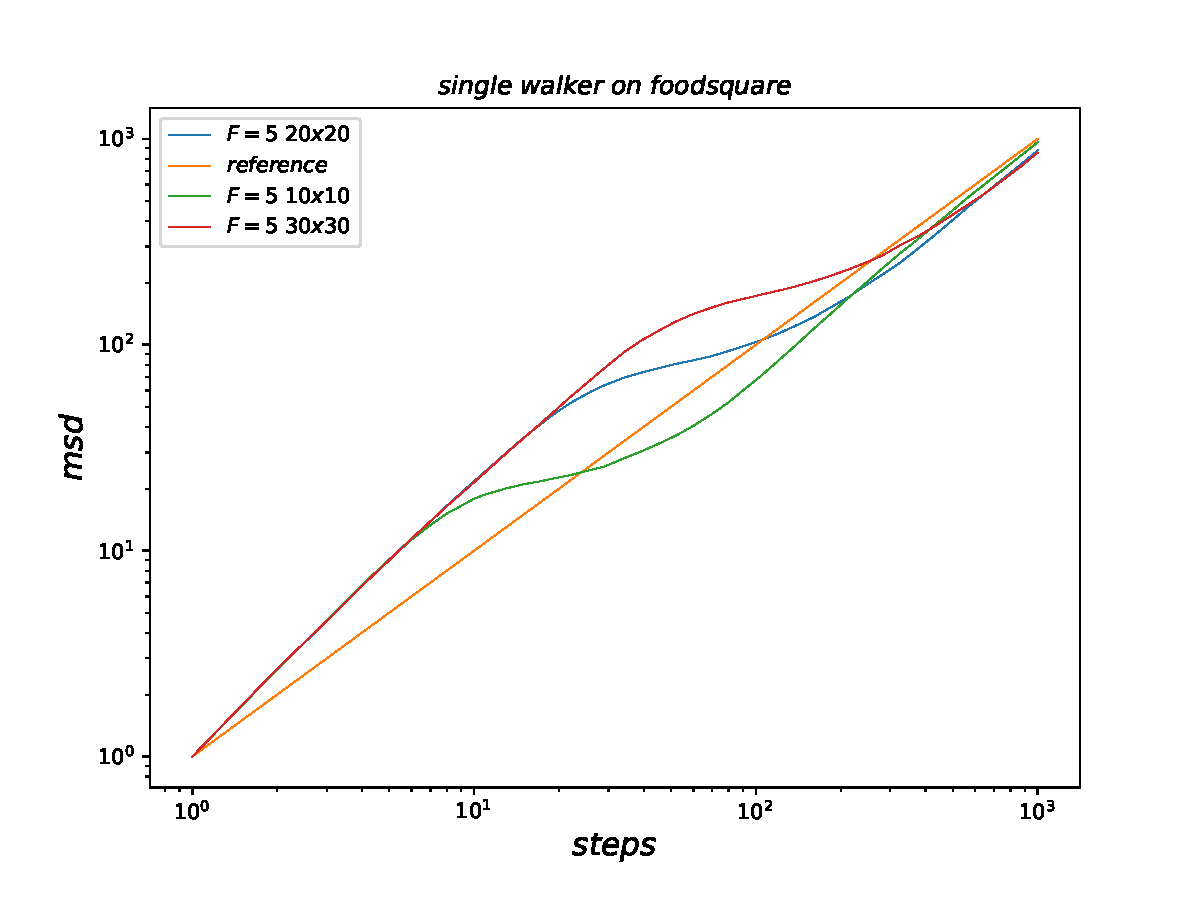
\includegraphics[scale=0.8]{abc.pdf}
	\caption{Ergebniss der MC-Simulation eines einzelnen Walkers auf Nahrungsquadraten unterschiedlicher Größe.}
\end{figure}

\newpage

\subsubsection{Einzelner Walker auf der Nahrungsmatrix bei fixem Startpunkt}

In diesem Unterkapitel soll das $msd$ eines einzelnen Walkers auf einer Nahrungsmatrix die vorher von vielen Walkern 'angefressen' worden ist betrachtet werden. 
Das $msd$ in der Standardkonfiguration von Boxlänge $L=100$ und $N=1000$ Walkern, sowie Nahrungsparameter $F=5$, ist nach bei $t=42$ MC-Schritten zum Beispiel im subdiffusiven Bereich. Zu diesem Zeitpunkt wird eine Nahrungsmatrix gespeichert und ich suche (durch anschauen) das Ende einer Fressspur. Dort werden die Läufe des einzelnen Walkers gestartet. 
In der nachfolgenden Abbildung sieht man die für die Simulation verwendete Matrix.



\noindent Es wird die am Punkt $x=49,\ y=65$ endende Fressspur als Startpunkt für die Simulation gewählt. Es wurde über $10^6$ Läufe gemittelt.
\\
Man sieht, dass $msd$ weißt einen 'kleinen Knick' auf an dem der Exponent der Dynamik kleiner ist als bei freier Diffusion, allerdings fällt das $msd$ nicht unter das der freien Diffusion. Das verhalten der Kurve ist jedoch ähnlich, sie steigt zunächst stark an, steigt dann deutlich wenier stark und danach steigt sie wieder stark an. Die (numerische) Ableitung und damit auch die Kurve des Diffusionsexponenten sieht daher der der vielen Walker auch ähnlich aus. Man sieht zudem, dass der Diffusionsexponent unter 1 fällt, für ein paar Schritte liegt als Subdiffusion vor. (Achtung: keine strenge Subdiffusion, da $msd$ nicht unter diffusiv fällt!)


\begin{figure}[H]
	\centering
	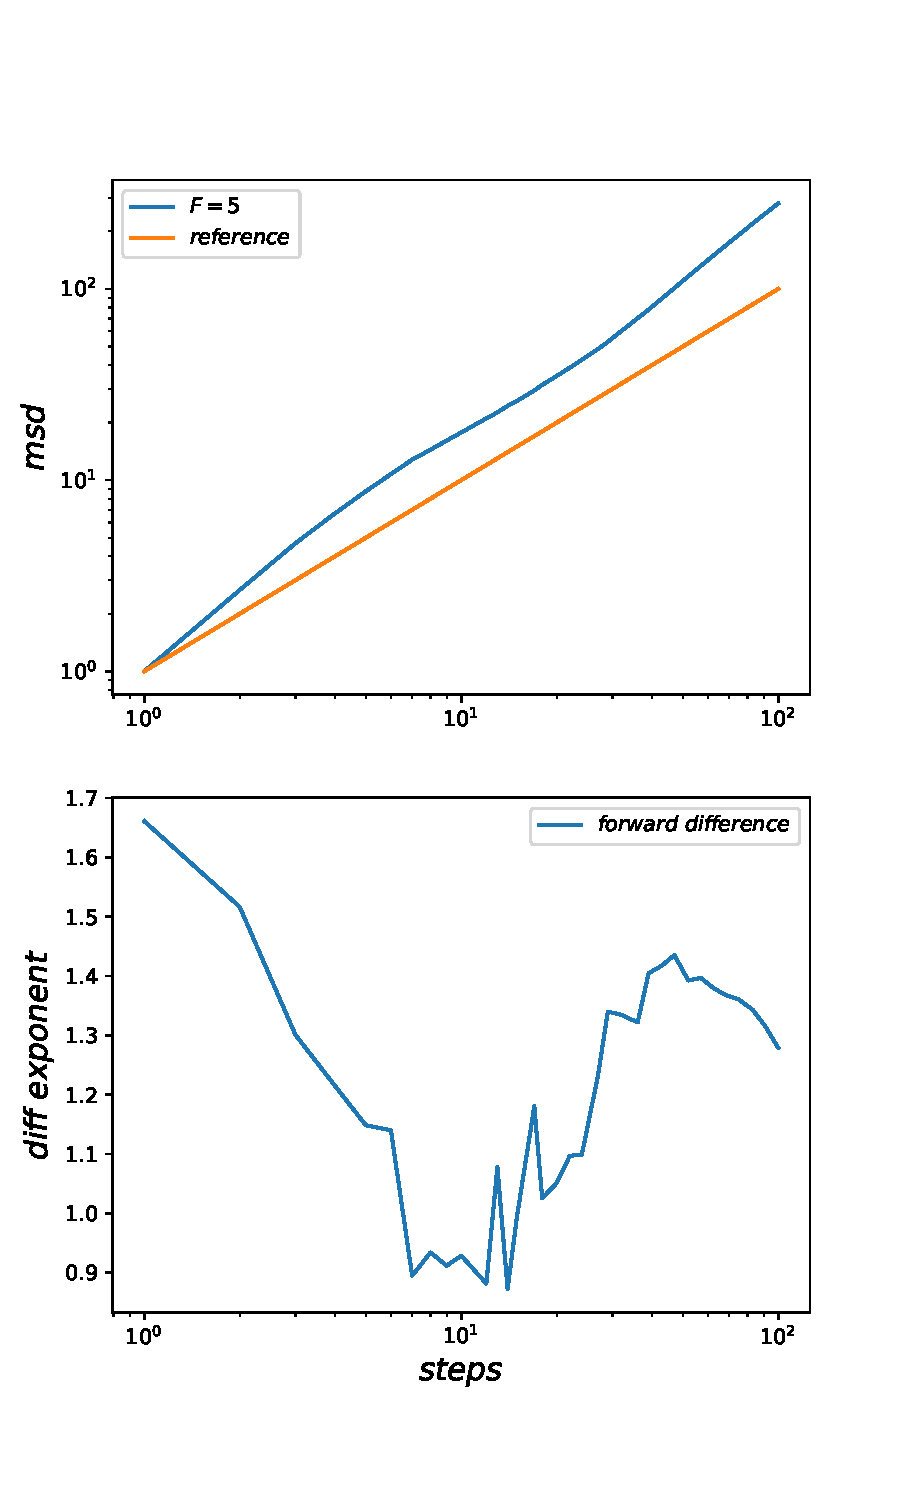
\includegraphics[scale=0.7]{single_walker_on_used_mat_nodisorderavg.pdf}
	\caption{Ergebniss der MC-Simulation eines einzelnen Walkers auf benutzter Nahrungsmatrix mit festem Startpunkt}
\end{figure}
\newpage

\subsubsection{Einzelner Walker auf der Nahrungsmatrix mit disorder-average}
Anders als im vorigen Unterkapitel wird nun der Startpunkt beliebig gewählt unter der Bedingung, dass von einem bereits besuchten Feld gestartet wird, dadurch wird über die Unordnung des Systems gemittelt ('disorder average'). Alternativ (oder zusätzlich) kann man auch über Nahrungsmatrizen mitteln, auch so ändert sich die Unordnung der Nahrung. 
\\
\noindent Es wird also versucht die Vielteilchendynamik auf eine Einteilchendynamik in einem 'effektiven Potential' zu übertragen. So kann herausgefunden werden ob die weitere Bewegung der anderen Random Walker auf dem bereits zerfallenen Nahrungsgitter noch den einen Walker beeinflusst.
\\
\noindent Man sieht keine Subdiffusion mehr, der Diffusionsexponent ist größer 1. Der Effekt verschwindet also durch den disorder-average. Der subdiffusive bereich war nur ein paar wenige Schritte lang. Wann die Subdiffusion eintritt ist stark von der disorder abhängig (vergleiche die unterschiedlich großen Nahrungsquadrate im Minimalmodell), mitteln wir über den Startpunkt so tritt dieser schwache subdiffusive Bereich immer zu anderer Zeit auf und mittelt sich weg.
\\
\noindent Es ist also die Bewegung der anderen Walker und die damit verbundene Veränderung der Nahrungsverteilung die diesen langen (streng) subdiffusiven Bereich hervorruft.

\begin{figure}[H]
	\centering
	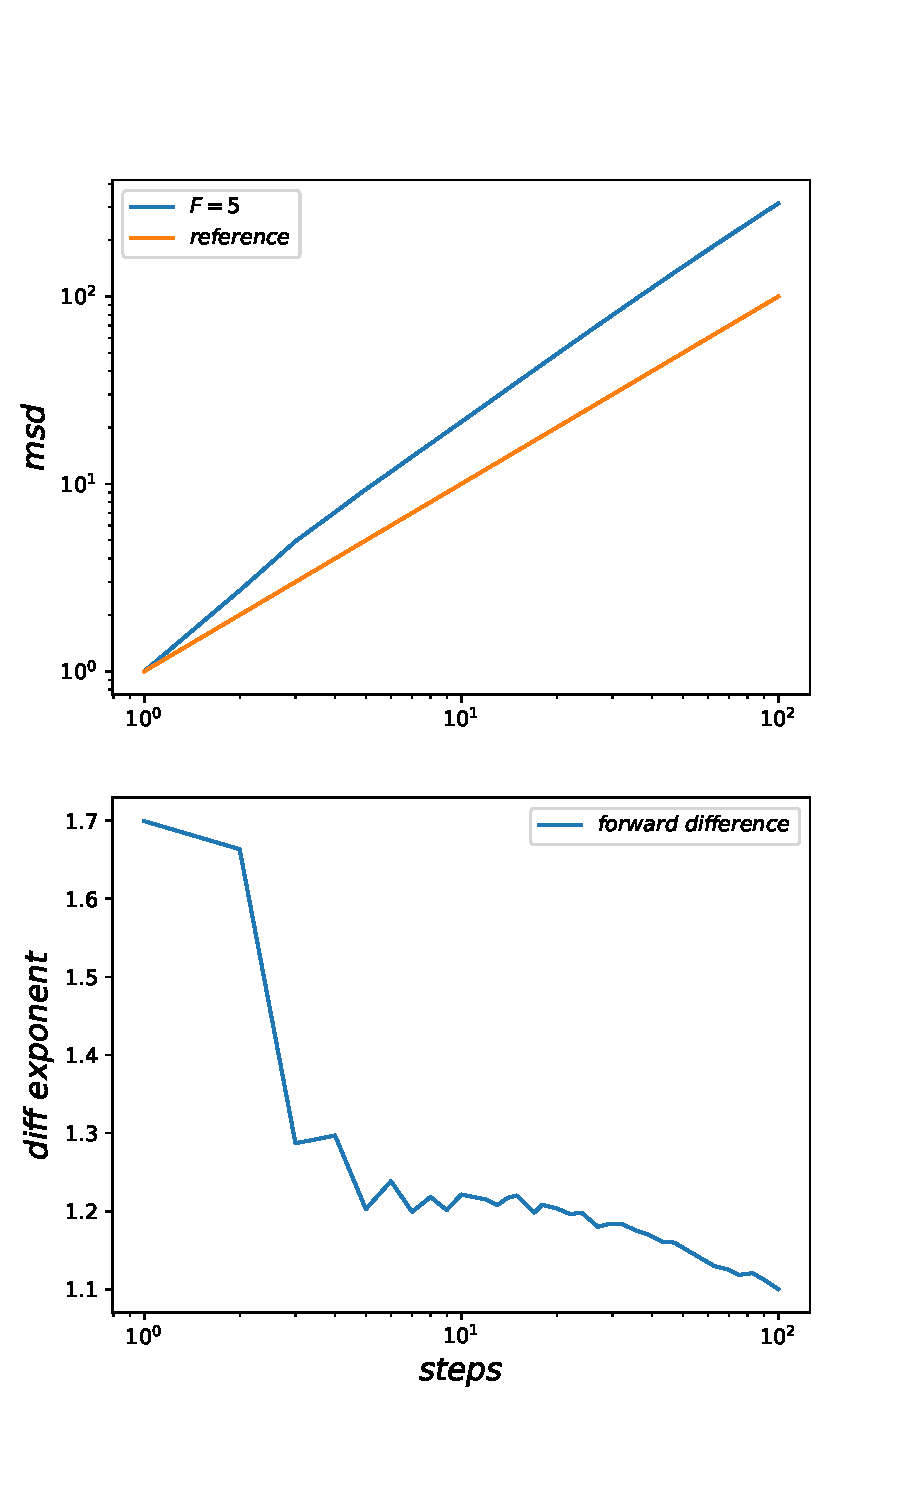
\includegraphics[scale=0.8]{single_walker_on_used_mat_disorderavg.pdf}
	\caption{Ergebniss der MC-Simulation eines einzelnen Walkers auf benutzter Nahrungsmatrix mit zufälligem zuvor besuchten Startpunkt}
\end{figure}

\newpage

\subsection{Unterschiedliche Walkerdichten und ihr Effekt auf die Dynamik}
In dem vorigen Abschnitt \ref{minimalmodell} wurde der Einfluss unterschiedlich großer Nahrungsquadrate auf die Dynamik des einzelnen Walkers gezeigt. Aus diesem Ergebniss kann man raten, dass eine höhere Dichte an Random Walkern einen ähnlichen Effekt auf die Vielteilchendynamik hat wie ein kleineres Nahrungsquadrat auf die Einteilchendynamik im Minimalmodell, denn je mehr Walker auf der Nahrungsmatrix sitzen, desto schneller und und kleinteiliger zerfällt das Nahrungsgitter. 
\\
Man erwartet also, das bei steigender Dichte das streng subdiffusive Verhalten nach weniger Schritten eintritt. Naiv ist aber nicht klar, ob die stärke des Effektes von der Walkerdichte abhängig ist, also ob der Diffusionsexponent unterschidlich weit sinkt oder nicht.
\\
\noindent
Die nachfolgende Grafik zeigt die Simulationsergebnisse ($msd$ und Diffusionsexponent) bei den Walkerdichten 5\%, 10\%, 20\% und 50\% auf der $100 \times 100$ Nahrungsmatrix, es wurde über 2000, 1000, 500, 200 Läufe gemittelt um immer über $10^6$ einzelne $msd$ zu mitteln.
\\
\noindent Die Simulationsergebnisse bestätigen eindeutig, dass der Eintritt der strengen Subdiffusion mit der Dichte in oben vermuteter Weise zusammenhängt. Zudem lässt sich auch am Minimum des Diffusionsexponenten (numerisch bestimmt mit der 'forward-differnence' Methode) eine Tendenz erkennen: mit steigender Walkerdichte senkt sich das Minimum im Diffusionsexponenten nach unten. Die stärke der Subdiffusion scheint also (in dem hier simulierten Bereich mittlerer Dichten) mit steigender Dichte zuzunehmen.

\begin{figure}[H]
	\centering
	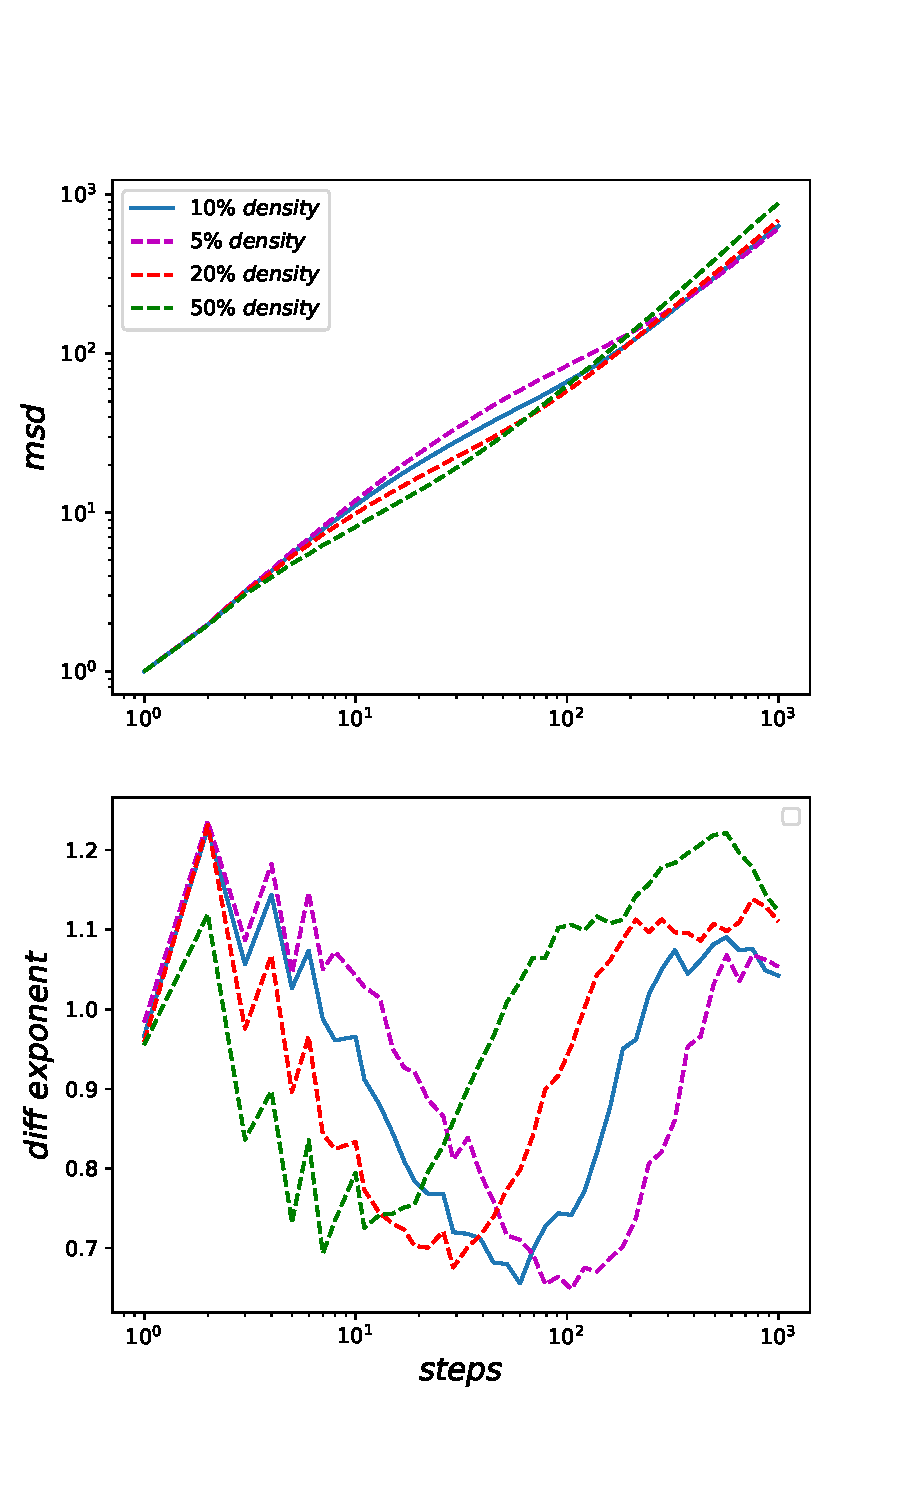
\includegraphics[scale=0.8]{alldens.pdf}
	\caption{Ergebniss der MC-Simulation bei unterschiedlichen Walkerdichten, es wurde in allen Kurven über $10^6$ einzelne $msd$ gemittelt.}
\end{figure}

\newpage
\section{Eindimensionales Modell}

\subsection{Mean Squared Displacement}

Um die bisherige Idee, dass die Ränder der verbliebenen Nahrungscluster die Dynamik in ein subdiffusives Regime bringen zu untermauern wird ein eindimensionales Modell betrachtet. In diesem Fall gibt es dementsprechend keine (wirklichen) Ränder, da diese nulldimensional sind, das Ablaufen eines Randes wie das Minimalmodell aus dem vorherigen Kapitel nahelegt ist daher nicht möglich. 
\\
Für die Simulation wird der gleiche Code wie bisher verwendet, also wird ebenfalls gleichzeitig und nach der selben Wahrscheinlichkeitsberechnung gezogen. 
\\
Klar ist, dass nach sehr langen Zeiten das $msd$ auf der Diffusionskurve ($F=0$) sein muss, da alle Nahrung weggessen ist und damit die Walker keine interaktion mehr haben und alle einen normalen eindimensionalen Random-Walk ausführen.
\\
Ebenfalls ist zu erwarten, dass am Anfang der Simulation die Walker stark superdiffusiv laufen müssen (bei $F=5$), da sie nahezu deterministisch in die Richtung des ersten Schrittes laufen müssen, denn es ist $\frac{e^5}{e^5 + 1} \approx 0.99$. 
\\
Kuezzeit- und Langzeitverhalten müssen daher mit dem zweidimensionalen Modell übereinstimmen, spannend ist also wie das verhalten auf mittlerer Zeitskala ist. Die entscheidende Frage lautet also: Gibt es ein subdiffusives Regime, in dem das $msd$ (bei $F=5$) unter der Diffusionskurve liegt? 

\begin{figure}[H]
	\centering
	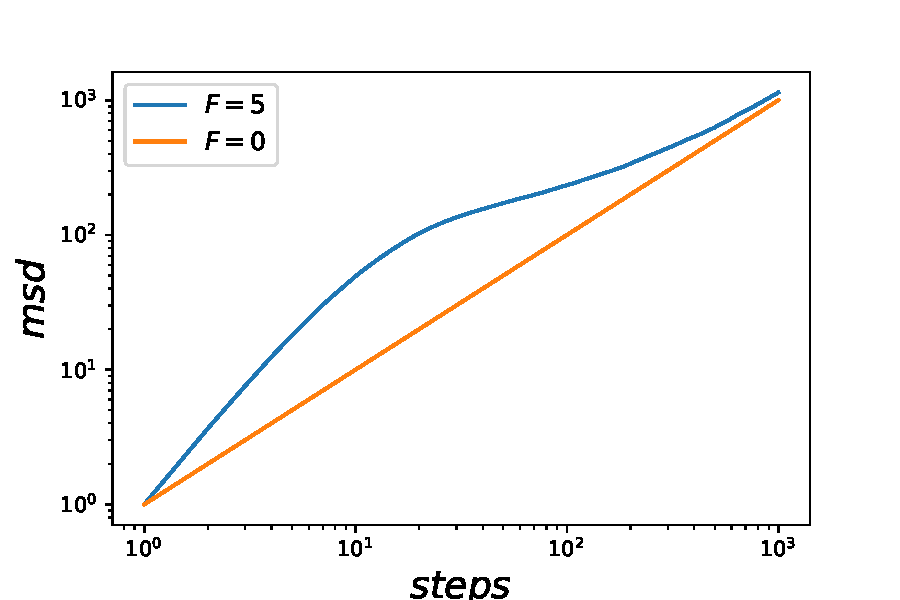
\includegraphics[scale=0.85]{onedmsd.pdf}
	\caption{Ergebniss der MC-Simulation des eindimensionalen Modells. Es wurde über 100 Läufe, also $10^4$ Samples gemittelt.}
\end{figure}

\newpage

\noindent Um Antwort auf diese Frage zu erhalten schaut man sich das Simulationsergebnis in der kommenden Abbildung an. Es gibt kein subdiffusives Regime, sondern nur ein superdiffusives zu Anfang, welches nach verschwinden der Nahrung sich auf die normale Diffusionskurve (von oben) anpasst.

\subsection{Autokorrelation der Schritte im eindimensionalen Modell}
Neben dem $msd$ kann erneut die Autokorrelation der Schritte $g_{t_0}(\tau)$ betrachtet werden. Aus dieser Größe kann man ablesen, wie stark der Schritt zur Zeit $t_0 + \tau$ mit dem Schritt zur Zeit $t_0$ korreliert ist.
\\
\noindent Es lässt sich eine längere Korrelation zum ersten Schritt vermuten, da bis zum erreichen der Fressspur eines benachbarten Walkers die Schritte nahezu deterministisch in die Richtung des ersten Schrittes erfolgen.
\\
\noindent In dem Plot der Autokorrelation der Schritte sieht man ganz deutlich, das der zweite Schritt noch sehr stark zum ersten Schritt korreliert ist. Dies ist im zweidimensionalen Modell nicht so gewesen. Die Erklärung dafür ist einfach, in zwei Dimensionen hat der Walker nach dem ersten Schritt (in den meisten Fällen bei 10\% Dichte) 3 Felder neben sich mit Nahrung die gleich Wahrscheinlich besucht werden, im eindimesionalen Fall nur ein Feld (das wo der Walker nicht her kommt) und daher ist die Korrelation zu Beginn stärker. 
\\
Dadurch ist auch klar, wieso das $msd$ zu Beginn stärker superdiffusiv ist.


\begin{figure}[h!]
	\centering
	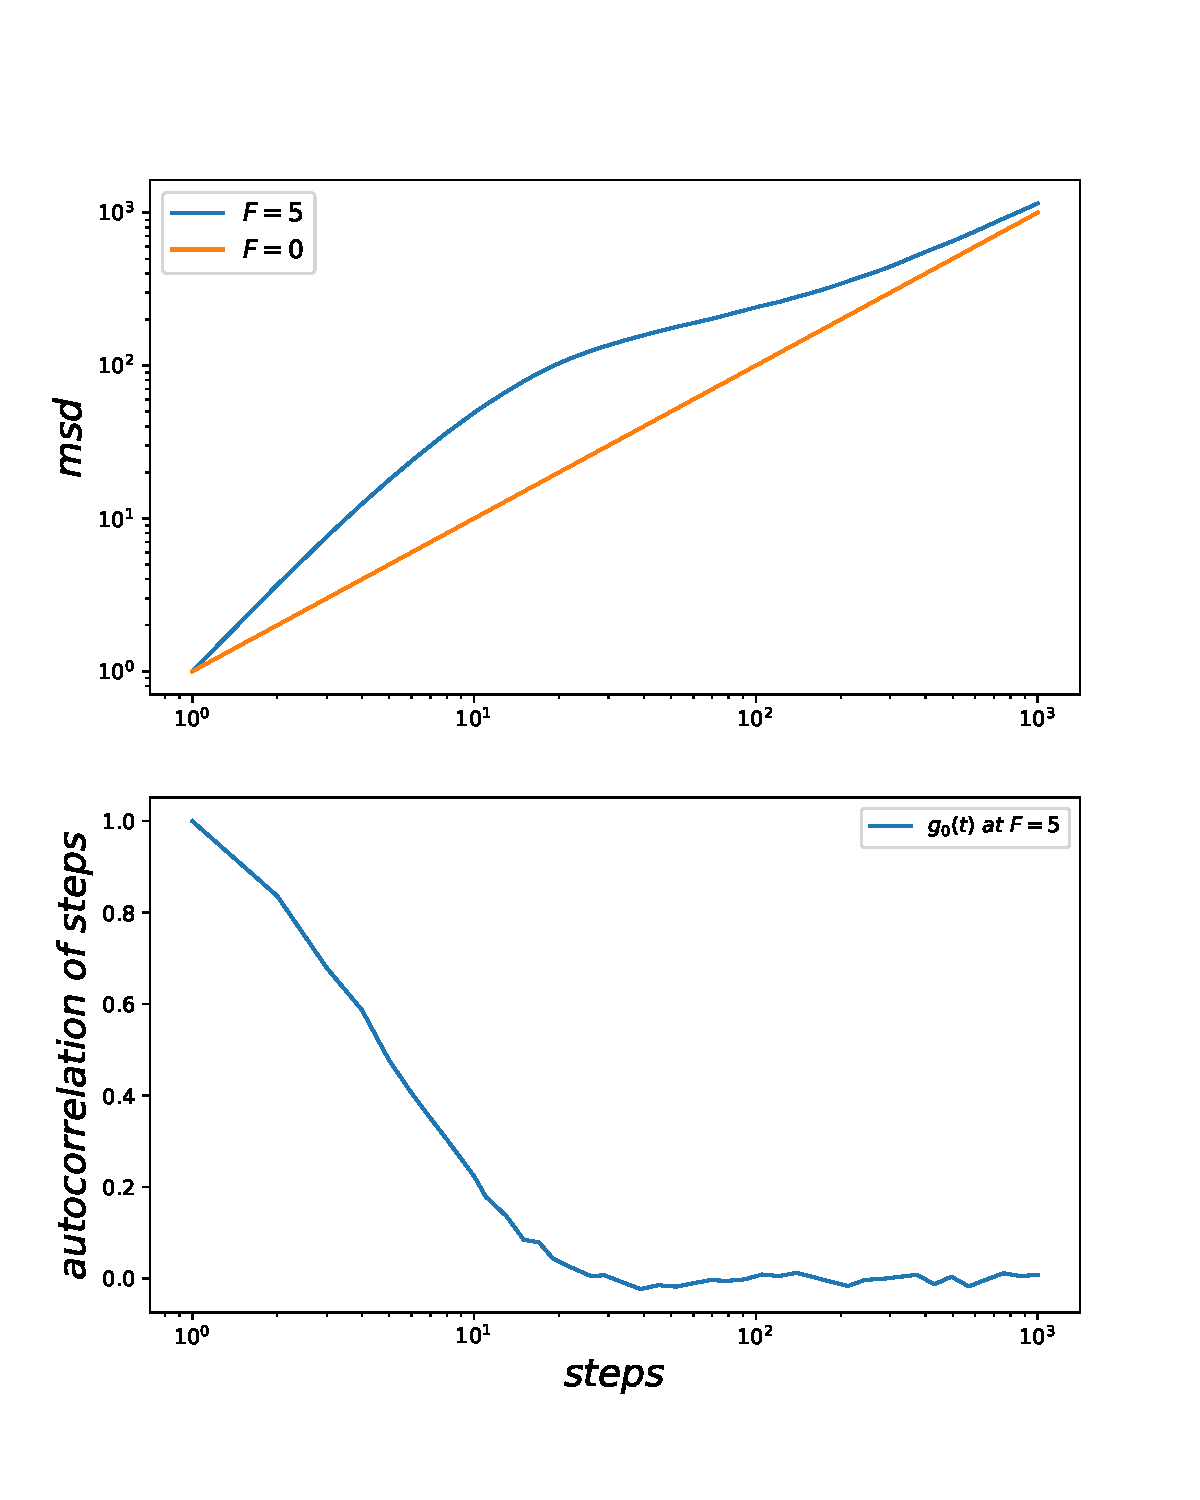
\includegraphics[scale=0.7]{onedescp.pdf}
	\caption{Autokorrelation der Schritte des eindimensionalen Modells. Es wurde über 100 Läufe, also $10^4$ Samples gemittelt.}
\end{figure}












\end{document}